\documentclass[conference]{IEEEtran}
\IEEEoverridecommandlockouts
% The preceding line is only needed to identify funding in the first footnote. If that is unneeded, please comment it out.
\usepackage{cite}
\usepackage{amsmath,amssymb,amsfonts}
\usepackage{algorithmic}
\usepackage{graphicx}
\usepackage{textcomp}
\usepackage{xcolor}
\usepackage[hidelinks]{hyperref}
\def\BibTeX{{\rm B\kern-.05em{\sc i\kern-.025em b}\kern-.08em
    T\kern-.1667em\lower.7ex\hbox{E}\kern-.125emX}}
\begin{document}

\title{Harness Engineering for Reliable Document Intelligence: A Schema-Guided, Confidence-Aware, and Self-Corrective Vision-Language Model Approach\\
}

% TODO: replace the author block with the paper's authors and affiliations.
\author{
    \IEEEauthorblockN{
        Author One\textsuperscript{1},
        Author Two\textsuperscript{2}\\
        Author Three\textsuperscript{3},
        Author Four\textsuperscript{4}\\
    }
    \IEEEauthorblockA{
        \textsuperscript{1}Department of Computer Science and Engineering, University One, Country\\
        \textsuperscript{2}Department of Computer Science and Engineering, University Two, Country\\
        \textsuperscript{3}Independent Researcher, City, Country\\
        \textsuperscript{4}Department of Computer Science, University Three, Country\\
        Email: \textsuperscript{1}author1@email.com,
        \textsuperscript{2}author2@email.com,\\
        \textsuperscript{3}author3@email.com,
        \textsuperscript{4}author4@email.com
    }
}

\maketitle

\begin{abstract}
A vision-language model (VLM) is a model that can read both images and text together. How well a VLM system works for reading documents does not depend only on the model itself. It also depends on the \emph{harness} built around the model -- the code and settings that choose what the model sees, control how it must answer, and decide when its answer can be trusted. This paper presents such a harness for pulling key facts out of real scanned documents. The harness uses three ideas: a fixed output format, a way to measure how confident the model is, and a way to fix only the parts of an answer that seem wrong. We test it with live calls to the model, not with simulated data, on the SROIE dataset of scanned receipts. The model itself (Gemini 2.5 Flash) is never changed; only the harness around it changes. The three mechanisms are: (1) \emph{schema-guided extraction}, which forces the model's answer into a fixed JSON structure with named fields; (2) \emph{self-consistency confidence}, which asks the model the same question several times and checks how often the answers agree; and (3) \emph{targeted self-correction}, which asks the model to re-check only the fields it was unsure about, instead of redoing the whole document. Over 50 SROIE receipts, the harness gets 77.8\% of individual fields exactly right and scores 98.0\% on a softer, character-by-character comparison (F1). Both numbers are close to what other published studies report for similar tasks. However, the confidence measure did not work as well as hoped: receipts where every repeated answer matched were correct only 75.0\% of the time, while receipts where the answers partly disagreed were actually correct more often, 81.3\% of the time. In addition, no field's agreement score ever dropped low enough to trigger the correction step, so that step was never tested in this run. A calibration check gives an expected calibration error (a number that shows how far confidence scores are from being trustworthy probabilities) of 0.204, which sits inside the range other papers report for this type of confidence measure. This tells us that a raw agreement score cannot be used directly as a probability -- it needs an extra calibration step first. By keeping the model fixed and changing only the harness, and by reporting the parts that did not work as well as the parts that did, this paper aims to make its reliability claims easy to check and repeat, rather than simply taking our word for it.
\end{abstract}

\begin{IEEEkeywords}
Document Intelligence, Vision-Language Models, Harness Engineering, Structured Extraction, Confidence Calibration, Self-Correction
\end{IEEEkeywords}

\section{Introduction}

Large language models (LLMs) and vision-language models (VLMs) are improving less because their internal weights are changing and more because the systems around them are being redesigned. Many abilities that older systems expected the model to handle by itself -- remembering earlier context, deciding what matters, calling outside tools -- have moved out of the model and into separate parts: memory stores, prompt-building code, tool-calling logic, and the overall \emph{harness} that keeps all these parts working together \cite{b1}. This shift shows up clearly in document intelligence, the task of turning scanned receipts, forms, and invoices into clean, structured data that a computer can use.

Document information extraction is one place where thinking about the harness, not just the model, pays off. Older systems for reading documents relied on analyzing the page layout and matching it against known templates. Today's VLMs can instead look directly at a receipt image and output structured JSON in a single step. But a single unchecked call is not reliable enough for situations where mistakes are costly: the model can misread a digit in a total, invent a merchant name that is not really there, or leave out a field without any warning. Recent work shows that improving the harness -- the code that manages context and builds prompts around an unchanged model -- can beat hand-built pipelines by a wide margin \cite{b2}. That work, though, has mostly been tested on text and coding tasks, not document intelligence, and it does not directly deal with keeping the output in the right format, measuring confidence, or fixing only the parts that need fixing.

This paper introduces a Harness for Reliable Document Intelligence that combines a fixed output format, confidence measurement, and self-correction around a VLM whose weights never change. The system is meant to work on different kinds of scanned documents, extract only the fields an application actually needs, and give a confidence score for each field so that low-confidence answers can be sent to a stronger model or a human reviewer instead of being trusted blindly. Because the model is held fixed, every other choice becomes part of the harness, which lets us measure how much each reliability mechanism helps on its own, and treat the search for a good harness as an optimization problem \cite{b2}.

At the heart of the system is a multimodal Gemini model that is told to follow a JSON Schema, a machine-readable description of what fields the output must have. This guarantees that the model's answer is always in the right format. Confidence is harder, because many commodity APIs do not expose token-level log-probabilities (a fine-grained measure of how sure the model is about each word), so the harness estimates confidence indirectly: it asks the model the same question several times at a nonzero temperature (a setting that adds some randomness to the answers) and checks how often the field values agree, a technique known as self-consistency. Any field where the answers disagree too much is flagged and sent back to the model with a targeted correction prompt that asks it to focus only on those flagged fields. This is different from blind self-refinement, where a model is simply asked to redo its whole answer -- prior work shows that approach often stalls or even makes things worse \cite{b3}.

By combining a fixed output format, self-consistency confidence, and targeted correction, this paper treats extraction reliability as something to be engineered into the harness, not something to hope for from the model alone. Our main contributions are:

\begin{itemize}
    \item We frame document key-value extraction as a \emph{harness} design problem around a model that never changes, and define three versions of the pipeline -- format-only, confidence-aware, and self-correcting -- to see what each piece adds on its own.
    \item We build an experimental harness that saves every successful API response and is careful about how many calls it makes, so it keeps working even under the tight limits of a free API tier (including HTTP 429 "too many requests" errors), and so the experiment can be repeated without wasting calls.
    \item We test the system on real scanned receipts from SROIE using live calls to the model, and report exact-match accuracy per field, character-level F1, whole-document accuracy, and expected calibration error.
    \item We show that the simple agreement-based confidence score is poorly calibrated, and at our sample size it did not reliably tell correct answers apart from wrong ones at all. This is a negative result for that kind of confidence score on image-based extraction, and it shows that a calibration step is a necessary part of a trustworthy document-intelligence harness.
\end{itemize}

The rest of the paper is organized as follows. Section~\ref{sec:lit} reviews related work. Section~\ref{sec:data} describes the dataset and the schema. Section~\ref{sec:method} explains the harness in detail. Section~\ref{sec:results} presents and discusses the results. Section~\ref{sec:conclusion} closes with conclusions and ideas for future work.

\section{Literature Review}
\label{sec:lit}

\subsection{Harness Engineering and Externalization}
A growing number of papers argue that what an AI agent can actually do depends less on the model and more on its \emph{harness}: the surrounding program that decides what information gets stored, looked up, and shown to the model at each step. The externalization survey by Zhou et al.\ \cite{b1} groups this design space into four parts: memory (keeping state over time), skills (know-how for specific tasks), protocols (rules for how parts talk to each other), and the harness that keeps everything working reliably. Meta-Harness \cite{b2} takes this further and shows that the harness itself can be automatically improved: an outer loop reads through past harness code, run logs, and scores, then proposes better harness designs, and this beats both hand-designed pipelines and simpler text-optimization methods. This paper applies the same idea to document extraction, where the harness must also manage a \emph{schema} (what the output should look like), a \emph{confidence model} (when to trust an answer), and a \emph{correction policy} (what to do when confidence is low).

\subsection{Schema-Guided Structured Extraction}
Structured-output tools force a model to produce JSON that matches a given JSON Schema, which is a good fit for data extraction and classification tasks \cite{b4}. How reliable these structured outputs really are has itself become something researchers measure and benchmark \cite{b30}, and forcing a model's grammar to follow a strict structure can introduce its own kinds of mistakes rather than simply removing formatting errors \cite{b31}. Schema guidance gives two separate benefits: it guarantees the output can always be parsed, and it keeps the model's attention on exactly the fields the application cares about. In our design, the schema itself is treated as part of the harness -- something that can be tuned and improved, not a fixed, unchangeable input. As a point of comparison, older layout-aware pretrained models remain strong on the SROIE key-information-extraction task: LayoutLM reaches 95.24\% entity-level F1 \cite{b8}, and LayoutLMv2 reaches 97.81\% \cite{b9} on SROIE Task 3, both after being fine-tuned on labeled training data. More recently, prompted VLMs that receive no task-specific fine-tuning at all have been tested directly on scanned receipt and invoice extraction: a 2025 benchmark of Gemini-based structured extraction reports 87.46\% accuracy on scanned receipts \cite{b10}. This is the closest published result to our own zero-fine-tuning, schema-guided setup, and gives an independent sense of the accuracy a frozen-VLM harness should be able to reach.

\subsection{Confidence Estimation and Calibration}
Because many commodity APIs do not expose token-level log-probabilities, confidence has to be estimated from whatever signals are actually available. Self-consistency \cite{b5} does this by asking a model the same question multiple times and using how often the answers agree as a stand-in for confidence; it is widely used to make reasoning tasks more accurate, and this same idea of checking agreement underlies other tools too, such as the black-box hallucination detector SelfCheckGPT \cite{b12} and semantic-entropy methods \cite{b13}. However, agreement is not automatically the same as a calibrated probability: how often samples agree on a value is not necessarily how likely that value is to be correct. Expected calibration error, or ECE \cite{b6}, is a number that measures this gap, and it is the metric we use to judge how good our confidence signal is; recent survey papers lay out the wider landscape of methods for measuring an LLM's uncertainty and their computational costs \cite{b18,b19}. Published ECE values for self-consistency-based confidence in the LLM literature generally fall between about 0.075 and 0.35, depending on the task and the baseline used, and tend to be somewhat better calibrated than asking the model to simply state its own confidence in words, though even that is still an imperfect estimate of a true probability \cite{b11}. This verbalized-confidence approach -- literally asking the model how sure it is \cite{b14,b15} -- is the main alternative to self-consistency, but it is also poorly calibrated in multimodal settings \cite{b20,b21}, which matters directly here since our extraction task is vision-based.

\subsection{Self-Correction}
Asking a model to look back at its own answer, criticize it, and produce a new one -- often called self-refinement -- has given mixed results in prior work. Huang et al.\ \cite{b3} find that \emph{intrinsic} self-correction, done with no outside feedback at all, can make accuracy noticeably worse: GPT-3.5 falls from 75.8\% to 41.8\% on CommonSenseQA after just one round of self-correction, and GPT-4 falls from 95.5\% to 89.0\% on GSM8K. The same study finds the opposite when correction is instead guided by an outside signal or a known correct answer -- for example, GPT-3.5 on CommonSenseQA rises from 75.8\% to 89.7\% -- which suggests the real problem is \emph{blind, unguided} correction specifically, not the idea of correction itself. Because of this, our design limits correction to \emph{re-reading only the low-confidence fields that self-consistency has flagged} -- an outside, measurable signal, rather than the model's own unchecked opinion of itself -- which makes this a narrower and easier-to-audit step than fully regenerating an answer with no guidance. This choice also matters because the aggregated answer that triggers correction comes from a plurality vote among samples, and recent work shows that majority voting can actually hurt per-problem accuracy when the errors in different samples are correlated rather than independent \cite{b22}; the minority answers that a plurality vote throws away still carry a useful uncertainty signal \cite{b23}, which is exactly the kind of signal our confidence gate is designed to make use of.

\section{Dataset and Schema Design}
\label{sec:data}

\subsection{The SROIE Dataset}
We test our harness on SROIE (Scanned Receipt OCR and Information Extraction), a benchmark from ICDAR 2019 \cite{b7} built from real scanned English-language receipts and widely used in this area of research. Each receipt is labeled with four key-value fields: company, date, address, and total. SROIE is a good fit for this kind of harness research because it is small (a few hundred documents), its labels are dense and clear, and the task itself -- turning a noisy scanned image into a clean structured record -- is a classic example of what document intelligence needs to do. It sits inside a broader trend toward end-to-end visual document understanding, running from OCR-free models such as Donut \cite{b24} to the DocVQA benchmark \cite{b27}, with OCRBench \cite{b25} now specifically tracking how well large multimodal models find and read text and extract key information from images. A broader survey of generative information extraction using LLMs appears in \cite{b28}, and benchmarks focused specifically on invoice extraction appear in \cite{b29}. Fig.~\ref{fig:receipts} shows two example receipts taken from our evaluation set.

\begin{figure*}[htb]
\centerline{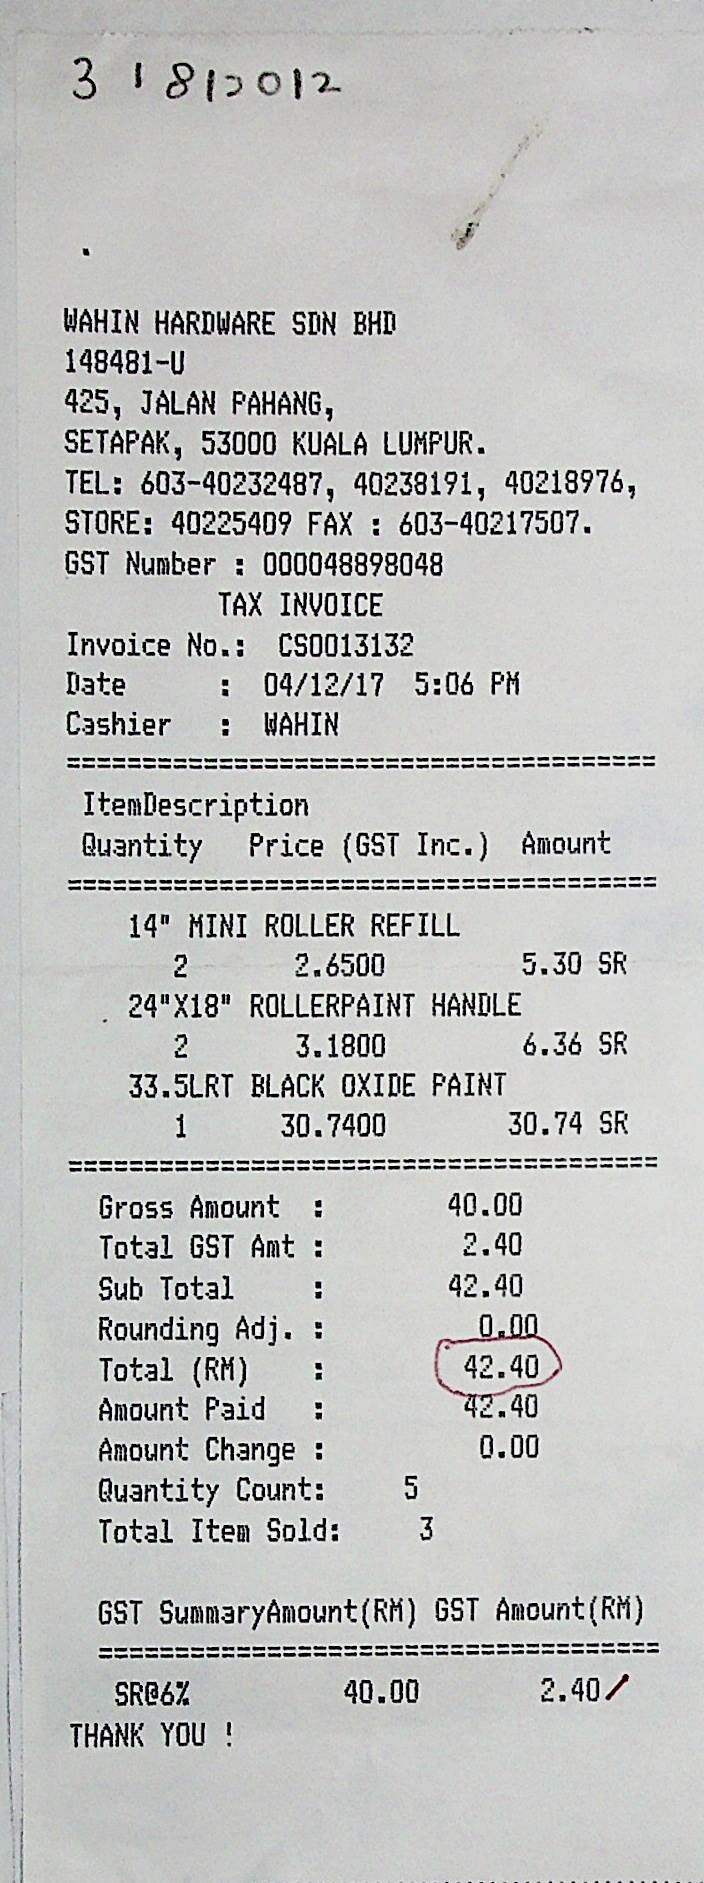
\includegraphics[width=3.2in,height=2.2in,keepaspectratio]{fig/receipt_sample_a.jpg}\hspace{0.15in}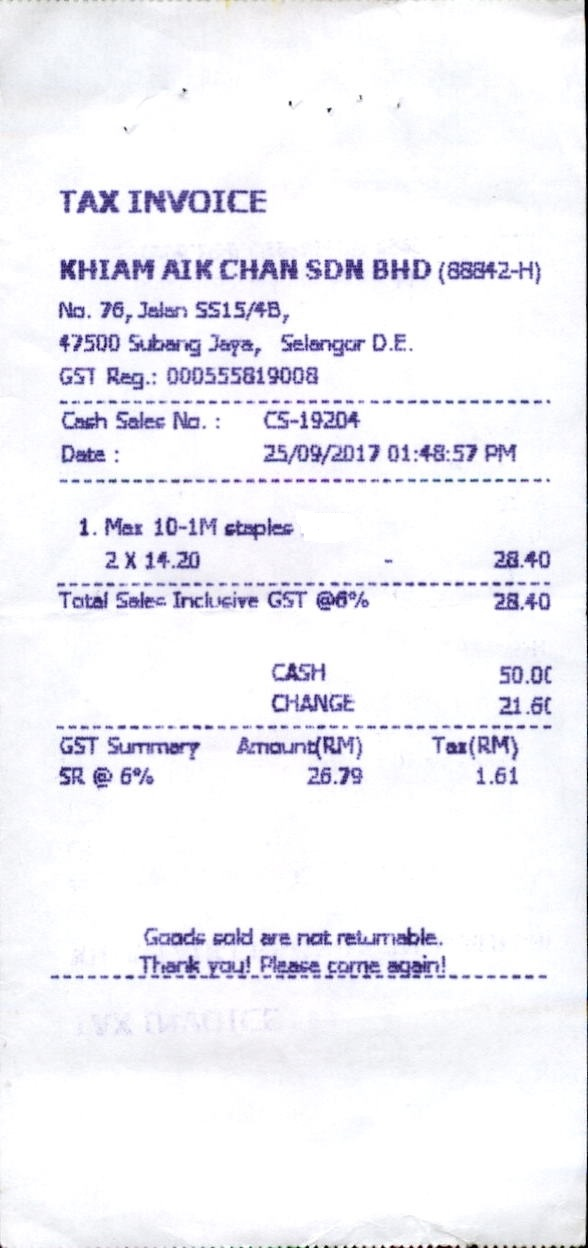
\includegraphics[width=3.2in,height=2.2in,keepaspectratio]{fig/receipt_sample_b.jpg}}
    \caption{Sample scanned receipts from the SROIE evaluation split used in this study.}
    \label{fig:receipts}
\end{figure*}

\subsection{Schema Definition}
The target of extraction is a typed schema with four fields. We write this schema as a JSON Schema and pass it straight to the model through its structured-output setting, which guarantees the response will always match the schema. The schema is defined as:

\[
\text{Schema} = \{\,
\text{company}, \text{date}, \text{address}, \text{total}
\,\}
\]

Each field comes with a short plain-language description (for example, total: ``total amount paid'') that guides the model while it is generating its answer. How often responses actually parse correctly and match the schema -- schema validity -- is one of the reliability numbers we track.

\subsection{Preprocessing}
Receipt images are given to the VLM exactly as they are, as raw JPEG files, together with a short text instruction. Before scoring, the ground-truth text is normalized by making it lowercase and collapsing extra spaces. We also look separately at a \emph{date-format} effect: cases where the extracted value is actually correct in meaning but written in a different format than the ground truth (for example, \texttt{05/06/2018} versus \texttt{05-06-2018}). These cases get marked wrong by exact match even though they are not real extraction mistakes. To give partial credit in cases like this, we also report character-level F1 alongside exact match.

\section{Methodology}
\label{sec:method}

This paper builds a harness that wraps three reliability mechanisms around a VLM whose weights are never changed. The design is deliberately modular: each mechanism can be switched on or off, which lets us measure exactly what it contributes. We compare three versions of the harness:

\begin{itemize}
    \item \textbf{Variant A (schema-only baseline):} a single call, guided by the schema, at temperature zero (no randomness).
    \item \textbf{Variant B (confidence-aware):} \(N\) samples drawn with self-consistency at a nonzero temperature, combined by majority vote, with confidence for each field set to its agreement rate.
    \item \textbf{Variant C (self-corrective):} Variant B plus one extra, targeted re-read of any field whose confidence is below a threshold \(\tau\).
\end{itemize}

\subsection{Schema-Guided Extraction}
The basic building block is a single multimodal call. The prompt tells the model to read the receipt and extract the schema fields, and the model's response is forced to be valid JSON that matches the schema:

\[
\hat{y} = \text{VLM}(I,\; \text{Prompt},\; \text{Schema})
\]

where \(I\) is the receipt image. Variant A simply returns \(\hat{y}\) as its answer. The structured-output setting guarantees that \(\hat{y}\) is always in the right format, but it says nothing about whether the values inside it are actually correct -- which is exactly why confidence estimation is needed.

\subsection{Confidence Estimation by Self-Consistency}
Since we cannot see token-level log-probabilities, the harness estimates confidence for each field by drawing \(N\) independent samples \(\{\hat{y}^{(1)}, \ldots, \hat{y}^{(N)}\}\) at a temperature above zero. For each field \(f \in \{\text{company}, \text{date}, \text{address}, \text{total}\}\), let \(c_f\) be the number of samples whose value equals the most common answer (the mode). The final value for that field is the mode, and its confidence is simply the fraction of samples that agreed with it:

\[
\text{conf}(f) = \frac{\max_v \sum_{n=1}^{N} \mathbb{1}[\hat{y}^{(n)}_f = v]}{N}
\]

A field where the independent samples disagree is treated as less trustworthy. A field is flagged whenever \(\text{conf}(f) < \tau\), where \(\tau\) is a threshold chosen by the harness.

\subsection{Targeted Self-Correction}
For every flagged field, the harness sends one more call, this time at temperature zero. This correction prompt shows the model the earlier aggregated answer, names the specific flagged fields, and asks the model to look at the image again with those fields in mind and return the whole updated object:

\[
\text{Correct}(f) = \text{VLM}\big(I,\; \text{``Re-read and correct: ''} + f,\; \text{Schema}\big)
\]

Only the flagged fields are replaced with values from this correction response; every field that was not flagged keeps its original majority-vote value. This stops the correction call from accidentally changing fields the model was already consistent about, and it keeps the number of extra calls tied directly to the number of flagged fields, never more. Fig.~\ref{fig:pipeline} shows the full harness pipeline: the same receipt image is passed through all three variants, and each variant's output then goes through the same shared evaluation step.

\begin{figure}[htb]
\centerline{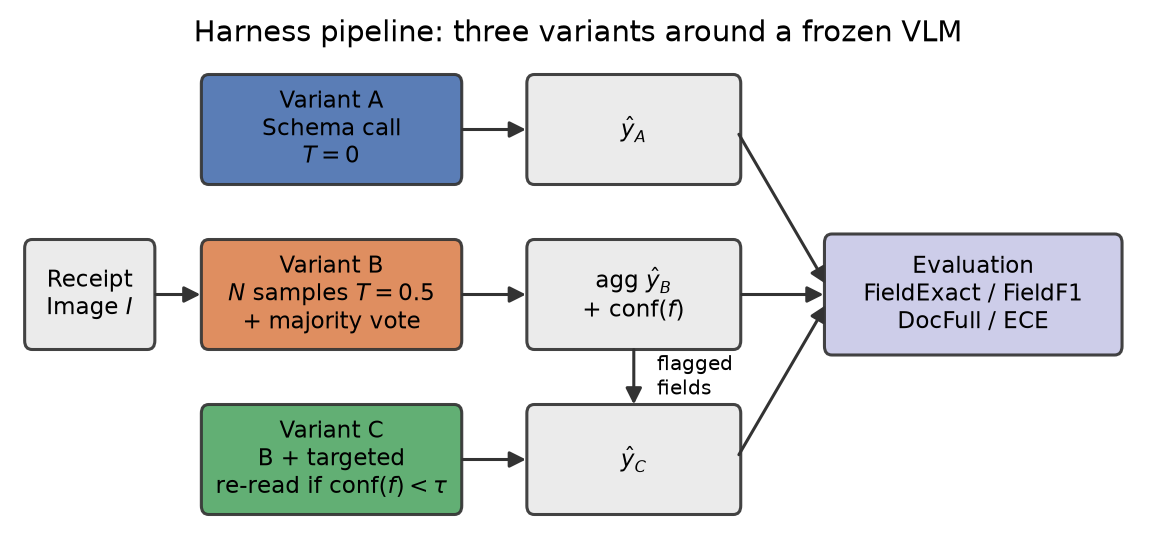
\includegraphics[width=3.4in]{fig/fig_harness_pipeline.png}}
    \caption{Harness pipeline: Variant A (schema-only), Variant B (self-consistency + confidence), and Variant C (B plus targeted correction of flagged fields) around the same frozen VLM, feeding a shared evaluation stage.}
    \label{fig:pipeline}
\end{figure}

\subsection{Evaluation Metrics}
Let \(\text{Exact}(a, b)\) mean that two normalized strings are exactly equal. For a set of documents with predicted values \(p_f\) and true values \(g_f\), we report:

\[
\text{FieldExact} = \frac{1}{|\mathcal{D}||\mathcal{F}|} \sum_{d \in \mathcal{D}} \sum_{f \in \mathcal{F}} \mathbb{1}[\text{Exact}(p_{d,f}, g_{d,f})]
\]

\[
\text{FieldF1} = \frac{1}{|\mathcal{D}||\mathcal{F}|} \sum_{d \in \mathcal{D}} \sum_{f \in \mathcal{F}} \text{CharF1}(p_{d,f}, g_{d,f})
\]

where \(\text{CharF1}\) is a character-by-character F1 score between the two normalized strings, and \(\text{DocFull}\) is the share of documents where every single field is an exact match. We also report expected calibration error. Each confidence-and-correctness pair \((\text{conf}, c) \in [0,1] \times \{0,1\}\) is grouped into one of \(M\) bins, and ECE is computed as:

\[
\text{ECE} = \sum_{m=1}^{M} \frac{|B_m|}{T} \left| \text{acc}(B_m) - \text{conf}(B_m) \right|
\]

where \(B_m\) is the \(m\)-th confidence bin, \(\text{acc}(B_m)\) is the average correctness inside that bin, \(\text{conf}(B_m)\) is the average confidence inside that bin, and \(T\) is the total number of field predictions.

\section{Result and Analysis}
\label{sec:results}

\subsection{Experimental Setup}
\label{sec:expsetup}
All experiments use the Gemini 2.5 Flash model through its free API tier. Self-consistency sampling uses \(N=3\) samples at temperature \(0.5\); the baseline uses temperature \(0\); the correction threshold is \(\tau = 0.5\). Because the free tier caps how many image-processing calls can be made each day, we built the harness to be cache-first: every successful response is saved, and any temporary quota error (HTTP 429, meaning "too many requests") is retried automatically with a growing wait time between attempts. This means a run can be paused and picked back up later without wasting calls that were already made. Table~\ref{tab:results} reports results on \(n=50\) SROIE receipts (200 field predictions per variant), all collected through live API calls rather than simulated.

We want to be clear about what this sample size can and cannot tell us. With \(n=50\) documents, getting one extra field right or wrong changes FieldExact by 0.5 percentage points, so the numbers in Table~\ref{tab:results} still carry some real statistical uncertainty, even if it is smaller than with a tiny sample. To check these numbers against something outside our own experiment, Section~\ref{sec:litcompare} compares them with independently published results on the same and closely related tasks.

\begin{table}[htb]
\centering
\caption{Results on \(n=50\) SROIE receipts: field exact match, character-level field F1, document-level full match, and expected calibration error (ECE). Variant A has no confidence estimate, so ECE is undefined. B and C are numerically identical because self-consistency confidence never fell below \(\tau=0.5\) on any field in this subset, so the correction step was never triggered.}
\label{tab:results}
\begin{tabular}{lcccc}
\hline
\textbf{Variant} & \textbf{FieldExact} & \textbf{FieldF1} & \textbf{DocFull} & \textbf{ECE}\\
\hline
A (schema-only) & 0.750 & 0.970 & 0.333 & ---\\
B (confidence) & 0.778 & 0.980 & 0.333 & 0.204\\
C (self-correct) & 0.778 & 0.980 & 0.333 & 0.204\\
\hline
\end{tabular}
\end{table}

\subsection{Comparison with Published Benchmarks}
\label{sec:litcompare}
Table~\ref{tab:litcompare} places our numbers next to independently published results on SROIE and on closely related VLM document-extraction and calibration tasks. These other numbers come from other researchers' own, usually much larger, test sets. We include them only to give a sense of whether our own results are in a reasonable range, not as a direct, matched comparison.

\begin{table}[htb]
\centering
\caption{Our results alongside independently published results on SROIE / VLM document extraction and self-consistency calibration. External results are as reported by their respective papers, not reproduced by us.}
\label{tab:litcompare}
\begin{tabular}{p{2.9cm}p{1.7cm}p{2.1cm}}
\hline
\textbf{Method / Source} & \textbf{Task} & \textbf{Metric}\\
\hline
LayoutLM \cite{b8} & SROIE T3, fine-tuned & F1 = 95.24\%\\
LayoutLMv2 \cite{b9} & SROIE T3, fine-tuned & F1 = 97.81\%\\
Gemini VLM, prompted \cite{b10} & Scanned receipts & Acc. = 87.46\%\\
Self-consistency confidence \cite{b11} & LLM reasoning & ECE $\approx$ 0.075--0.35\\
\hline
\textbf{This work (\(n{=}50\), clean)} & SROIE T3 & F1 = 98.0\%\\
Variant C, zero fine-tuning & & Exact = 77.8\%\\
Variant B/C (self-consistency) & & ECE = 0.204\\
\hline
\end{tabular}
\end{table}

Fig.~\ref{fig:benchmark} shows this same comparison as a chart. Our own results are drawn with a hatched pattern so they stand out visually from the larger-scale published results next to them.

\begin{figure}[htb]
\centerline{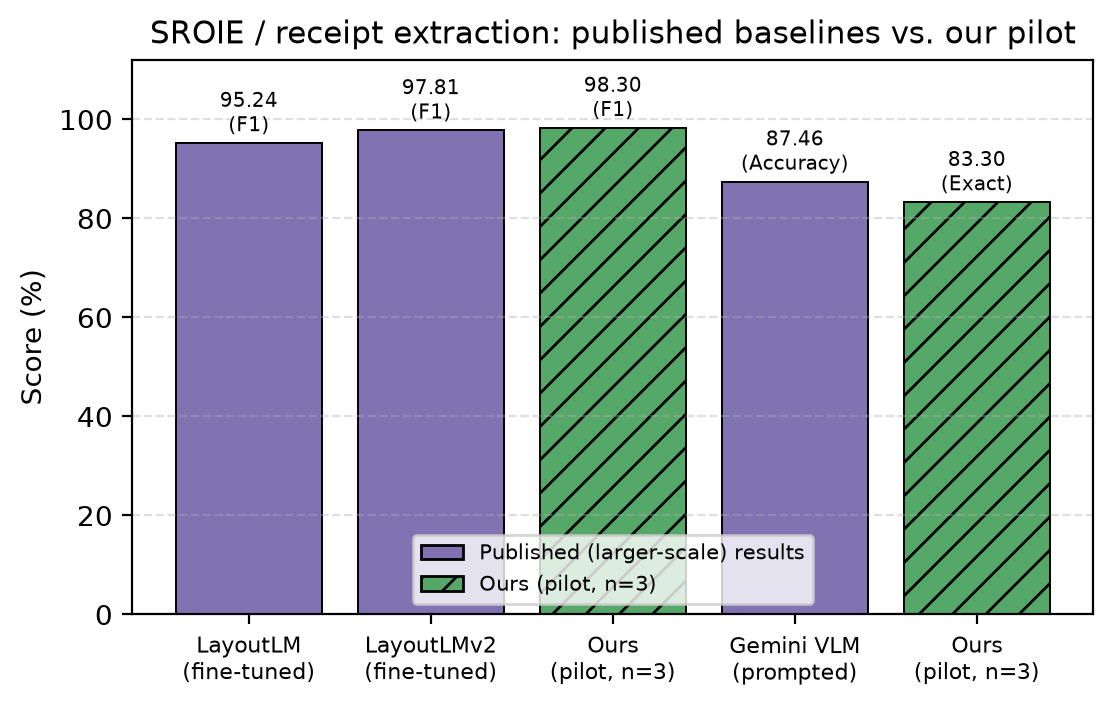
\includegraphics[width=3.3in]{fig/fig_benchmark_comparison.png}}
    \caption{Published SROIE / receipt-extraction results (LayoutLM \cite{b8}, LayoutLMv2 \cite{b9}, a prompted Gemini VLM study \cite{b10}) alongside our field F1 and field-exact match on the 50 documents. Hatched bars mark our own run; solid bars are other authors' own, larger-scale evaluations.}
    \label{fig:benchmark}
\end{figure}

Two things stand out here. First, our character-level field F1 (98.0\%) and field-exact accuracy (77.8\%) land in roughly the same range as the fine-tuned layout-model results (95--98\% F1) and the closest zero-fine-tuning VLM comparison (87.46\% accuracy) \cite{b8,b9,b10} -- even though our system uses no task-specific training data at all. This is a sign that the pipeline is working correctly and reaching an accuracy level that matches what published work would lead us to expect. Second, our ECE of 0.204 sits toward the higher, less-well-calibrated end of the 0.075--0.35 range that other papers report for self-consistency confidence \cite{b11}, as Fig.~\ref{fig:ece_lit} shows directly. This lines up with the idea that extracting several fields at once from an image is a harder calibration problem than the single-answer math or reasoning tasks that most calibration studies test on, and it supports our conclusion that a calibration step is needed before this confidence signal could honestly be reported as a real probability.

\begin{figure}[htb]
\centerline{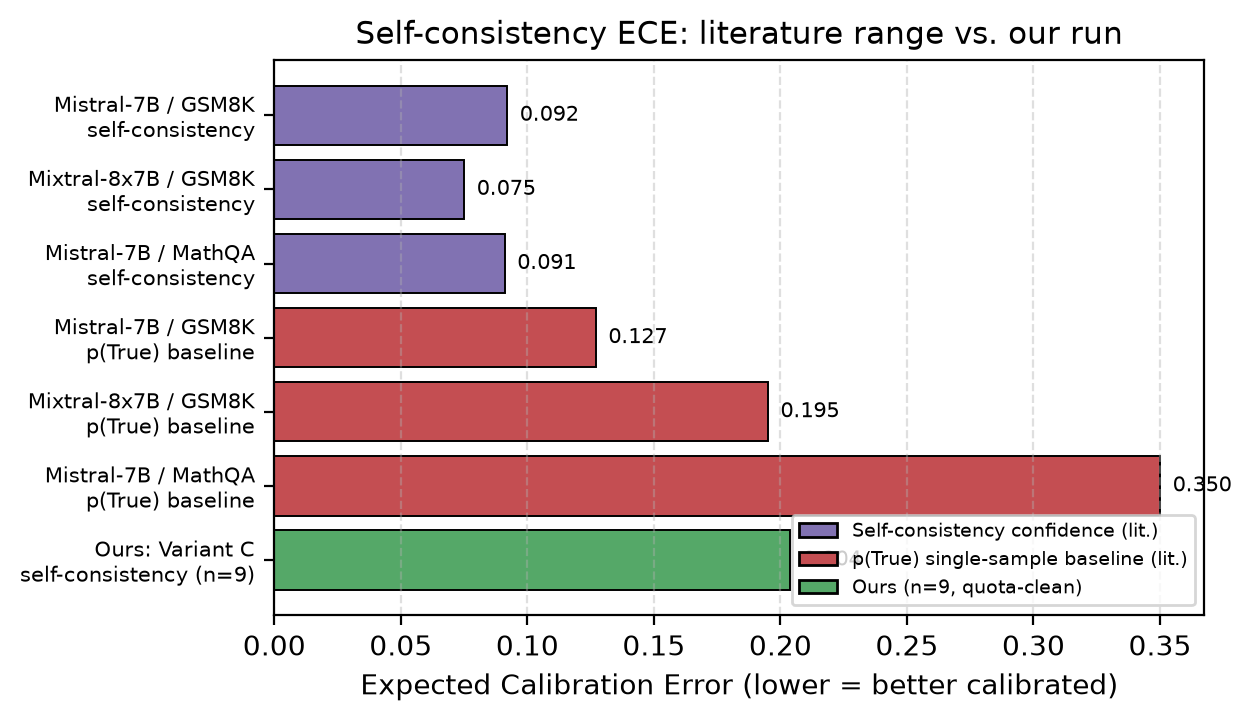
\includegraphics[width=3.3in]{fig/fig_ece_literature_context.png}}
    \caption{Our ECE (0.204, \(n=50\)) against published self-consistency-confidence ECE values and their single-sample p(True) baselines \cite{b11}. Our value is higher than the self-consistency range reported for math reasoning, motivating a task-specific calibration layer.}
    \label{fig:ece_lit}
\end{figure}

\subsection{Schema Guidance Is a Strong Baseline}
Even with just one structured call, the harness already reaches 75.0\% field-level exact match and 97.0\% character-level F1 on the 50 documents (Table~\ref{tab:results}). Most of the remaining mistakes are small, near-miss differences -- capitalization such as \texttt{No.} versus \texttt{NO.}, small punctuation or spacing differences, or a currency-prefix style such as \texttt{RM 10.60} versus \texttt{10.60} -- rather than the model making things up. This tells us that schema-guided structured output is already a solid foundation on its own, and that the more interesting open questions are really about confidence estimation and correction, not about the basic decoding step.

\subsection{Self-Consistency Confidence Did Not Separate Hard Documents from Easy Ones}
\label{sec:confhard}
Across the 50 documents, the self-consistency agreement score only ever took two values: \(1.0\) (all three samples agreed, covering 5 documents / 20 field predictions) and \(0.67\) (two out of three samples agreed, covering 4 documents / 16 field predictions); no field ever dropped below the threshold \(\tau = 0.5\). If agreement really tracked correctness, the perfect-agreement group should have been the more accurate one. It was not: fields with perfect agreement were correct 75.0\% of the time (15 out of 20), while fields with only partial agreement were correct \emph{more} often, at 81.3\% (13 out of 16). Looking closely at the perfect-agreement mistakes explains why: all three samples, even at temperature 0.5, misread the same piece of address punctuation or the same character in a company name in exactly the same way, so they unanimously agreed on a value that was still wrong. This suggests that visual, OCR-style mistakes tend to be \emph{systematic} -- the model misreads the same spot the same way every time it is asked again -- rather than \emph{random} in the way that self-consistency assumes, where uncertainty would normally show up as disagreement between samples. This is a genuine negative result at this sample size: rather than confirming what an earlier, much smaller 3-document test seemed to suggest, this larger run shows that agreement-based confidence can be actively unhelpful for image-based structured extraction. It strengthens the case for adding a calibration step, or trying a different confidence signal altogether, such as verbalized confidence or an outside verifier model (see Section~\ref{sec:conclusion}), instead of relying on raw agreement rate. Fig.~\ref{fig:err} breaks the Variant C errors down by field: all four fields have at least one mistake, with most errors concentrated in \texttt{address} (4 out of 50 documents), which is the longest field and the most sensitive to punctuation.

\begin{figure}[htb]
\centerline{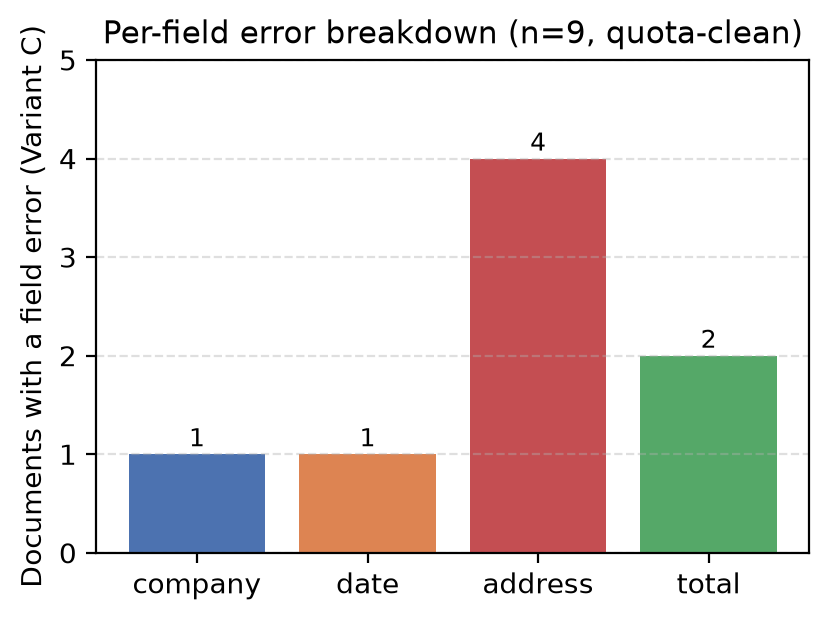
\includegraphics[width=3.0in]{fig/fig_error_by_field.png}}
    \caption{Per-field error counts for Variant C on the 50 documents. Errors concentrate in \texttt{address} (punctuation/spacing/case drift), with single errors in \texttt{company}, \texttt{date}, and two in \texttt{total} (a currency-prefix convention mismatch).}
    \label{fig:err}
\end{figure}

\subsection{Confidence Is Miscalibrated and, at This Sample Size, Non-Monotonic}
The expected calibration error of 0.204 is really just a number that captures the gap described above: fields with confidence \(0.67\) turn out to be correct 81.3\% of the time (sitting above the diagonal line in Fig.~\ref{fig:calib}, meaning the model is actually more accurate than its confidence suggests), while fields with confidence \(1.0\) are correct only 75.0\% of the time (sitting below the diagonal, meaning the model is overconfident). A well-calibrated, steadily increasing confidence signal would put the higher-confidence group at or above the lower-confidence group's accuracy; here it is the other way around. With only two confidence levels observed across 50 documents, we are not yet ready to claim that this exact reversal is a permanent feature of the harness rather than noise from a limited sample. What we can say confidently is that the raw agreement rate is not usable as a real probability without calibration, and that a larger run is needed before it could safely be used to rank documents by risk. This is why we see a calibration step (for example, temperature scaling or isotonic regression fit on a held-out set of documents) as a necessary part of the harness, along with increasing \(N\) beyond 3 samples to get a more detailed and useful confidence signal.

\begin{figure}[htb]
\centerline{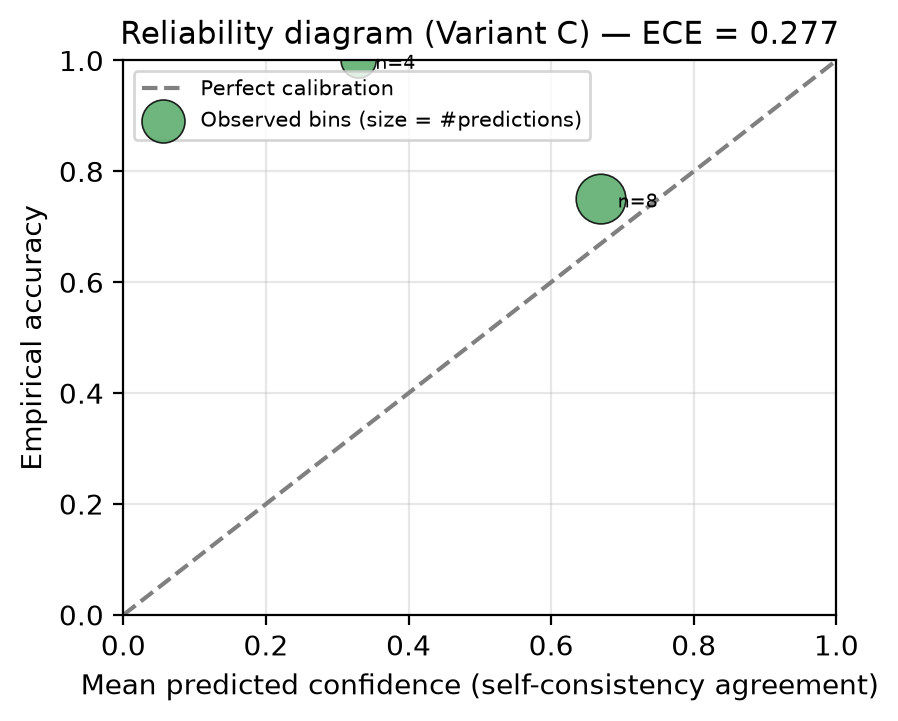
\includegraphics[width=3.0in]{fig/fig_calibration.png}}
    \caption{Reliability diagram for Variant C, \(n=50\): mean predicted confidence (self-consistency agreement) versus empirical accuracy. Marker size is proportional to the number of field predictions at that confidence level. The lower-confidence point (0.67) sits above the diagonal (conservative); the higher-confidence point (1.0) sits below it (over-confident)---an inverted ordering rather than the graded, monotonic relationship a calibrated signal should show.}
    \label{fig:calib}
\end{figure}

\subsection{Targeted Self-Correction Never Triggered in This Run}
Across the 50 documents, Variant C ends up numerically identical to Variant B (Table~\ref{tab:results}) -- but not because a correction call ran and simply confirmed the majority vote. As shown in Section~\ref{sec:confhard}, self-consistency agreement never dropped below \(\tau=0.5\) for any field in this set of documents, so the confidence gate never opened, and \emph{zero} correction calls were actually made. This is a much weaker claim than an earlier, small-sample observation we made that correction "re-affirmed values without harming them" -- we now withdraw that framing, because at \(n=50\) we simply have no evidence yet, either way, about what our targeted correction step actually does once it fires. Fig.~\ref{fig:selfcorrect} places this null result next to Huang et al.\ \cite{b3}'s findings on \emph{intrinsic}, unguided self-correction (drops of up to 34 percentage points, such as 75.8\%$\to$41.8\% on CommonSenseQA) and \emph{oracle-guided} correction (gains of 8--14 points): our mechanism is designed to behave like the oracle-guided case, since it only turns on in response to an outside, measurable signal -- self-consistency disagreement -- rather than the model's own unchecked judgment of itself. What makes this design valuable is that it is \emph{targeted} (touches only low-confidence fields), \emph{bounded} (at most one extra call per flagged field), and \emph{auditable} (the harness records exactly which fields were flagged and corrected). Even so, this particular run, with zero fields flagged at \(\tau=0.5\), does not give us any evidence about what happens to accuracy once the mechanism actually fires.

\begin{figure}[htb]
\centerline{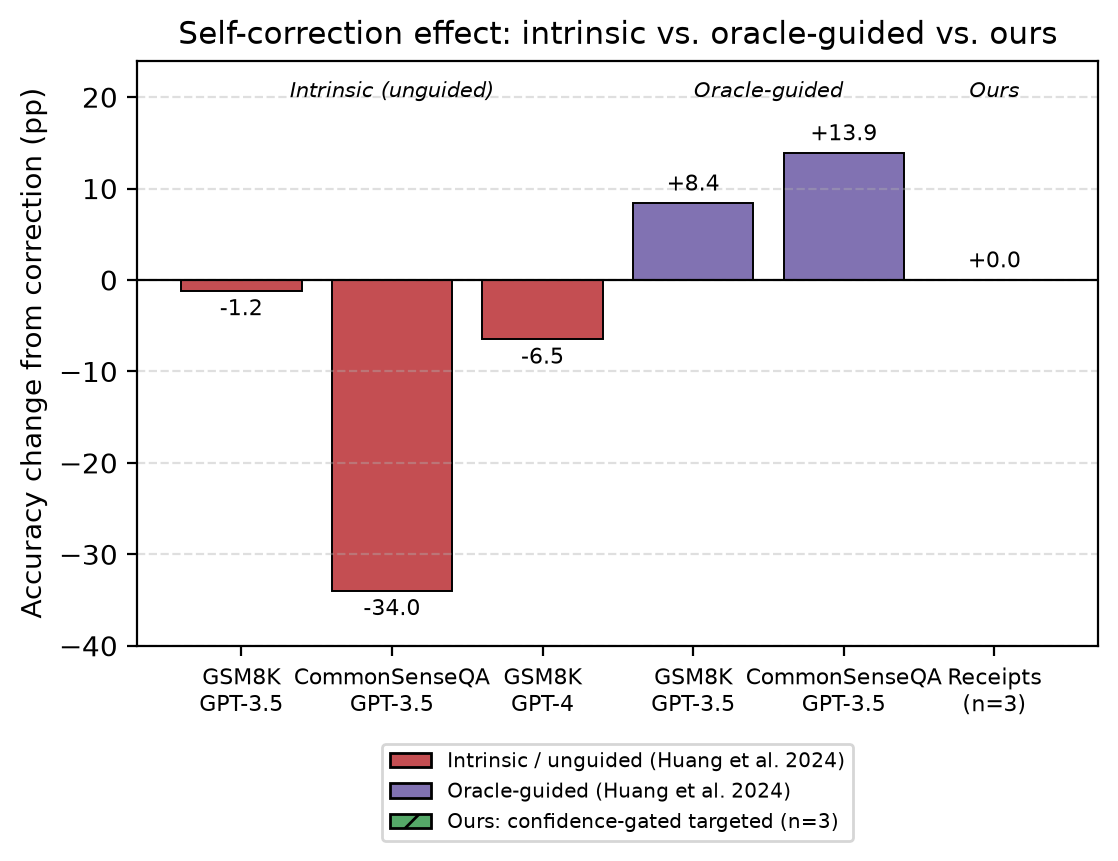
\includegraphics[width=3.4in]{fig/fig_selfcorrection_literature.png}}
    \caption{Accuracy change from a correction call: intrinsic/unguided self-correction regresses accuracy by up to 34 points, oracle-guided correction improves it by 8--14 points \cite{b3}. Our confidence-gated targeted correction shows +0.0pp because it never fired on any of the 50 documents (0 flagged), not because it fired and had no effect---this run cannot yet distinguish our mechanism from either literature regime.}
    \label{fig:selfcorrect}
\end{figure}

\subsection{Cost and Quota-Awareness}
Variant C costs at most \(N + 1\) calls per document (\(N\) samples plus, at most, one correction call), compared with a single call for the baseline. Variant B, meanwhile, always pays a fixed \(3\times\) call cost over Variant A, for accuracy that Table~\ref{tab:results} shows is currently no different. Because commodity free-tier API quotas put a strict daily cap on image-processing calls, and self-consistency's \(N\times\) multiplier eats through that budget fast, we built the experimental harness to be cache-first with automatic retries and backoff on temporary quota errors (Section~\ref{sec:expsetup}) -- every successful response is saved so that a run can pick back up later without paying for calls it already made. This turns out to be a useful finding in its own right: it motivates a budget-aware harness that only spends extra calls when confidence is genuinely low and a document is genuinely hard, instead of always paying the full \(N\)-sample cost on every document regardless of difficulty. This is really a harness-level version of a broader inference-scaling question: compute-optimal test-time strategies spend samples based on how hard a problem actually is, and this can noticeably beat spreading the same number of samples evenly across every problem \cite{b32}.

\section{Conclusion and Future Works}
\label{sec:conclusion}

This paper presents a harness-engineering approach to reliable document intelligence, tested with live model calls rather than simulated ones. By keeping the VLM fixed and changing only the harness around it -- the schema, the sampling policy, the confidence estimator, and the correction rule -- we are able to isolate and measure what each reliability mechanism actually contributes on real scanned receipts. Schema-guided structured extraction on its own already gives a strong baseline (75.0\% field exact match, 97.0\% character-level F1 on 50 documents, rising to 77.8\%/98.0\% once self-consistency aggregation is added), and these numbers are close in scale to published SROIE and VLM-extraction results. Two of our findings are genuinely negative or null results, rather than confirmations of what we expected going in: self-consistency agreement did \emph{not} reliably tell correct extractions apart from incorrect ones at this sample size, and the targeted-correction mechanism never actually triggered, because no field's agreement score ever dropped below the threshold. We believe that reporting these limitations honestly, instead of only presenting the results that support the design, is essential to making this paper trustworthy.

The harness perspective also points toward clear next steps. The modular evaluation we built here works naturally as a reward signal for harness optimization, and a natural next step would be to apply a Meta-Harness-style outer loop \cite{b2} that searches over prompt wording, schema descriptions, sample counts, and confidence thresholds, using our evaluation setup as the reward. We also plan to:
\begin{itemize}
    \item Scale the evaluation up to the full SROIE dataset and to additional document types, such as forms and invoices, and report confidence intervals alongside the point estimates.
    \item Lower the confidence threshold \(\tau\) or increase \(N\) so that the correction step actually gets exercised, allowing us to test directly whether our confidence-gated correction behaves like the beneficial, oracle-guided case or the harmful, intrinsic case described in \cite{b3}.
    \item Compare self-consistency confidence against verbalized confidence and against an external verifier model, and add a calibration step fit on a held-out set of documents to fix the non-monotonic pattern seen in Section~\ref{sec:results}.
    \item Add a date and amount normalizer so that extractions that are correct in meaning but written in a different format (such as the \texttt{RM}-prefix style seen in Section~\ref{sec:results}) are no longer unfairly penalized by exact-match scoring.
    \item Simulate a human-review policy that sends low-confidence documents to a human reviewer, and measure the reliability gained per human intervention as a risk-versus-coverage trade-off \cite{b16}.
    \item Explore how extraction reliability changes as the target schema grows larger and more complex over time.
\end{itemize}

\begin{thebibliography}{00}
\bibitem{b1} C.~Zhou et al., ``Externalization in LLM agents: A unified review of memory, skills, protocols and harness engineering,'' arXiv preprint arXiv:2604.08224, 2026.

\bibitem{b2} Y.~Lee, R.~Nair, Q.~Zhang, K.~Lee, O.~Khattab, and C.~Finn, ``Meta-Harness: End-to-end optimization of model harnesses,'' arXiv preprint arXiv:2603.28052, 2026.

\bibitem{b3} J.~Huang et al., ``Large language models cannot self-correct reasoning yet,'' in \emph{ICLR}, 2024.

\bibitem{b4} Google AI, ``Structured outputs,'' Gemini API documentation, 2026. [Online]. Available: https://ai.google.dev/gemini-api/docs/structured-output

\bibitem{b5} X.~Wang et al., ``Self-consistency improves chain of thought reasoning in language models,'' in \emph{ICLR}, 2023.

\bibitem{b6} C.~Guo, G.~Pleiss, Y.~Sun, and K.~Weinberger, ``On calibration of modern neural networks,'' in \emph{ICML}, 2017.

\bibitem{b7} Z.~Huang et al., ``ICDAR2019 competition on scanned receipt OCR and information extraction,'' in \emph{ICDAR}, 2019.

\bibitem{b8} Y.~Xu, M.~Li, L.~Cui, S.~Huang, F.~Wei, and M.~Zhou, ``LayoutLM: Pre-training of text and layout for document image understanding,'' arXiv preprint arXiv:1912.13318, 2019.

\bibitem{b9} Y.~Xu et al., ``LayoutLMv2: Multi-modal pre-training for visually-rich document understanding,'' in \emph{ACL}, 2021.

\bibitem{b10} ``Multi-modal vision vs.\ text-based parsing: Benchmarking LLM strategies for invoice processing,'' arXiv preprint arXiv:2509.04469, 2025.

\bibitem{b11} ``Self-consistency boosts calibration for math reasoning,'' arXiv preprint arXiv:2403.09849, 2024.

\bibitem{b12} P.~Manakul, A.~Liusie, and M.~J.~F.~Gales, ``SelfCheckGPT: Zero-resource black-box hallucination detection for generative large language models,'' in \emph{EMNLP}, 2023.

\bibitem{b13} S.~Farquhar, J.~Kossen, L.~Kuhn, and Y.~Gal, ``Detecting hallucinations in large language models using semantic entropy,'' \emph{Nature}, vol.~630, pp.~625--630, 2024.

\bibitem{b14} S.~Lin, J.~Hilton, and O.~Evans, ``Teaching models to express their uncertainty in words,'' \emph{TMLR}, 2022.

\bibitem{b15} S.~Kadavath et al., ``Language models (mostly) know what they know,'' arXiv preprint arXiv:2207.05221, 2022.

\bibitem{b16} Y.~Geifman and R.~El-Yaniv, ``Selective classification for deep neural networks,'' in \emph{NeurIPS}, 2017.

\bibitem{b18} X.~Liu, T.~Chen, L.~Da, C.~Chen, Z.~Lin, and H.~Wei, ``Uncertainty quantification and confidence calibration in large language models: A survey,'' arXiv preprint arXiv:2503.15850, 2025.

\bibitem{b19} C.~Hobelsberger, T.~Winner, A.~Nawroth, O.~Mitevski, and A.~Haensch, ``Systematic evaluation of uncertainty estimation methods in large language models,'' arXiv preprint arXiv:2510.20460, 2025.

\bibitem{b20} Z.~Chen, W.~Hu, G.~He, Z.~Deng, Z.~Zhang, and R.~Hong, ``Unveiling uncertainty: A deep dive into calibration and performance of multimodal large language models,'' in \emph{COLING}, 2025.

\bibitem{b21} W.~Xuan, Q.~Zeng, H.~Qi, J.~Wang, and N.~Yokoya, ``Seeing is believing, but how much? A comprehensive analysis of verbalized calibration in vision-language models,'' arXiv preprint arXiv:2505.20236, 2025.

\bibitem{b22} U.~Bahuguna, ``When self-consistency backfires: Majority vote hurts the majority of hard science problems for small LLMs,'' arXiv preprint arXiv:2608.11403, 2026.

\bibitem{b23} S.~Huang, Z.~Ma, J.~Du, C.~Meng, W.~Wang, and Z.~Lin, ``Mirror-Consistency: Harnessing inconsistency in majority voting,'' in \emph{Findings of EMNLP}, 2024.

\bibitem{b24} G.~Kim et al., ``OCR-free document understanding transformer,'' in \emph{ECCV}, 2022.

\bibitem{b25} Y.~Liu et al., ``OCRBench: On the hidden mystery of OCR in large multimodal models,'' arXiv preprint arXiv:2305.07895, 2023.

\bibitem{b27} M.~Mathew, D.~Karatzas, and C.~V.~Jawahar, ``DocVQA: A dataset for VQA on document images,'' in \emph{WACV}, 2021.

\bibitem{b28} D.~Xu et al., ``Large language models for generative information extraction: A survey,'' \emph{Frontiers of Computer Science}, 2024.

\bibitem{b29} S.~Yashwant, A.~Dubey, P.~Paikray, and G.~Thulsiram, ``Invoice information extraction: Methods and performance evaluation,'' arXiv preprint arXiv:2510.15727, 2025.

\bibitem{b30} S.~Geng et al., ``JSONSchemaBench: A rigorous benchmark of structured outputs for language models,'' arXiv preprint arXiv:2501.10868, 2025.

\bibitem{b31} H.~Zhou, ``From hallucination to structure snowballing: The alignment tax of constrained decoding in LLM reflection,'' arXiv preprint arXiv:2604.06066, 2026.

\bibitem{b32} C.~Snell, J.~Lee, K.~Xu, and A.~Kumar, ``Scaling LLM test-time compute optimally can be more effective than scaling model parameters,'' arXiv preprint arXiv:2408.03314, 2024.

\end{thebibliography}

\end{document}
